\documentclass[12pt]{article}

\usepackage[utf8]{inputenc}
\usepackage{geometry}
\geometry{
    a4paper,
    total={170mm,257mm},
    left=25mm,
    right=25mm,
    top=25mm,
    bottom=25mm,
}
\usepackage{multicol}
\usepackage[font=small,labelfont=bf]{caption}
\setlength{\columnsep}{0.25cm}
\usepackage[inline]{enumitem}
\usepackage{amssymb}
\usepackage{xcolor}
\usepackage{mathtools} 
\setlength{\parindent}{0em}
\setlength{\parsep}{0em}
\usepackage{tikz}
\setlength{\parskip}{0em}
\usetikzlibrary{decorations.pathmorphing,patterns}
\usepackage[american,cuteinductors]{circuitikz}
\usetikzlibrary{shapes,arrows,circuits,calc,babel}
% Definition of blocks:
\tikzset{%
  block/.style    = {draw, thick, rectangle, minimum height = 3em,
    minimum width = 3em},
  sum/.style      = {draw, circle, node distance = 2cm}, % Adder
  input/.style    = {coordinate}, % Input
  output/.style   = {coordinate} % Output
}
% Defining string as labels of certain blocks.
\newcommand{\suma}{\Large$+$}
\newcommand{\inte}{$\displaystyle \int$}
\newcommand{\derv}{\huge$\frac{d}{dt}$}

\def\mf{\ensuremath\mathbf}
\def\mb{\ensuremath\mathbb}
\def\mc{\ensuremath\mathcal}
\def\lp{\ensuremath\left(}
\def\rp{\ensuremath\right)}
\def\lv{\ensuremath\left\lvert}
\def\rv{\ensuremath\right\rvert}
\def\lV{\ensuremath\left\lVert}
\def\rV{\ensuremath\right\rVert}
\def\lc{\ensuremath\left\{}
\def\rc{\ensuremath\right\}}
\def\ls{\ensuremath\left[}
\def\rs{\ensuremath\right]}
\def\bmx{\ensuremath\begin{bmatrix*}[r]}
\def\emx{\ensuremath\end{bmatrix*}}
\def\bmxc{\ensuremath\begin{bmatrix*}[c]}
\def\emxc{\ensuremath\end{bmatrix*}}
% \def\t{\lp t\rp}
% \def\k{\ls k\rs}

\newcommand{\demoex}[2]{\onslide<#1->\begin{color}{black!60} #2 \end{color}}
\newcommand{\demoexc}[3]{\onslide<#1->\begin{color}{#2} #3 \end{color}}
\newcommand{\anim}[3]{\onslide<#1->{\begin{color}{#2!60} #3 \end{color}}}
\newcommand{\ct}[1]{\lp #1\rp}
\newcommand{\dt}[1]{\ls #1\rs}

% \renewcommand{\familydefault}{\sfdefault}

\begin{document}
\begin{center}
\begin{Large}
\textbf{Applied Linear Algebra in Data Analaysis}\\
\vspace{0.1cm}
\textbf{Solutions to Linear Equations Assignment}
\end{Large}
\end{center}
\hrule
\vspace{0.2cm}

\begin{enumerate}
\item Derive force and displacement relationship for a series of $n+1$ springs (with spring constants $k_i$) connected in a line. There are $n$ nodes, with $f_i$ and $x_i$ representing the force applied and resulting displacement at the $i^{th}$ node. 
\begin{center}
    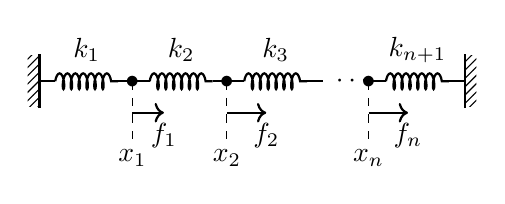
\begin{tikzpicture}
        \fill [pattern = north east lines] (-0.15,-0.325) rectangle (0,0.325);
        \draw[thick] (0,-0.34) -- (0,0.34);

        \draw[thick] (0,0) -- (0.2,0);
        \draw[decoration={aspect=0.3, segment length=1mm, amplitude=1mm, coil,},decorate, thick] (0.2,0) -- (1.0,0);
        \draw[thick] (1.0,0) -- (1.2,0);
        \node[black] at (1.18,-0.02) {$\bullet$};
        \node[black] at (0.6,0.4) {$k_1$};
        \draw[dashed, thin] (1.18,0) -- (1.18,-0.75) node[below]{$x_1$};
        \draw[->,thick] (1.18,-0.4) -- (1.58,-0.4) node[below]{$f_1$};

        
        \draw[thick] (1.2,0) -- (1.4,0);
        \draw[decoration={aspect=0.3, segment length=1mm, amplitude=1mm, coil,},decorate, thick] (1.4,0) -- (2.2,0);
        \draw[thick] (2.2,0) -- (2.4,0);
        \node[black] at (2.38,-0.02) {$\bullet$};
        \node[black] at (1.8,0.4) {$k_2$};
        \draw[dashed, thin] (2.38,0) -- (2.38,-0.75) node[below]{$x_2$};
        \draw[->,thick] (2.38,-0.4) -- (2.88,-0.4) node[below]{$f_2$};
        
        \draw[thick] (2.4,0) -- (2.6,0);
        \draw[decoration={aspect=0.3, segment length=1mm, amplitude=1mm, coil,},decorate, thick] (2.6,0) -- (3.4,0);
        \draw[thick] (3.4,0) -- (3.6,0);
        \node[black] at (3.0,0.4) {$k_3$};

        \node[black] at (4.0, 0) {$\cdots$};

        \draw[thick] (4.2,0) -- (4.4,0);
        \draw[decoration={aspect=0.3, segment length=1mm, amplitude=1mm, coil,},decorate, thick] (4.4,0) -- (5.2,0);
        \draw[thick] (5.2,0) -- (5.4,0);
        \node[black] at (4.18,-0.02) {$\bullet$};
        \node[black] at (4.8,0.4) {$k_{n+1}$};
        \draw[dashed, thin] (4.18,0) -- (4.18,-0.75) node[below]{$x_n$};
        \draw[->,thick] (4.18,-0.4) -- (4.68,-0.4) node[below]{$f_n$};

        \fill [pattern = north east lines] (5.4,-0.325) rectangle (5.55,0.325);
        \draw[thick] (5.4,-0.34) -- (5.4,0.34);
    \end{tikzpicture}
\end{center}
\begin{enumerate}
    \item Represent the relationship in the following form,
    \[ \mf{f} = \mf{Kx}; \,\,\, \mf{f} = \begin{bmatrix}f_1\\ f_2\\ \vdots\\ f_n\end{bmatrix}; \,\,\, \mf{x} = \begin{bmatrix}x_1 \\ x_2 \\ \vdots \\ x_n\end{bmatrix}\]
    \item What kind of a pattern does $\mf{K}$ have?
    \item Consider a specific case where $n = 4$ and $k = 1.5 N.m^{-1}$. What should be forces applied at the four nodes in order to displace the spring $\mf{x} = \begin{bmatrix*} 0.5 \\ -0.5 \\ 0 \\ 0 \end{bmatrix*}m$. 
\end{enumerate}

\item Consider the following electrical circuit with rectangular grid of resistors $R$. The input to this grid is a set of current injected at the top node as shown in the figure, such that $\sum_{k=1}^5i_k = 0$.
\vspace{-0.25cm}
\begin{center}
\begin{circuitikz}[scale=0.9]
    \draw (2,0) to[R,*-*] (0,0)
    to[R,*-*] (0,2) to[R,*-*] (0,4) to[R,*-*] (2,4)
    to[R,*-*] (2,2) to[R,*-*] (2,0) to[R,*-*] (4,0)
    to[R,*-*] (4,2) to[R,*-*] (4,4) to[R,*-*] (6,4)
    to[R,*-*] (6,2) to[R,*-*] (6,0) to[R,*-*] (8,0)
    to[R,*-*] (8,2) to[R,*-*] (8,4) to[R,*-*] (6,4);

    \draw (0,2) to[R,*-*] (2,2);
    \draw (2,4) to[R,*-*] (4,4);
    \draw (2,2) to[R,*-*] (4,2);
    \draw (4,2) to[R,*-*] (6,2);
    \draw (4,0) to[R,*-*] (6,0);
    \draw (6,2) to[R,*-*] (8,2);

    \draw (0,5) node[above]{$i_1$} to[short, o-] (0,4);
    \draw (2,5) node[above]{$i_2$} to[short, o-] (2,4);
    \draw (4,5) node[above]{$i_3$} to[short, o-] (4,4);
    \draw (6,5) node[above]{$i_4$} to[short, o-] (6,4);
    \draw (8,5) node[above]{$i_5$} to[short, o-] (8,4);
\end{circuitikz}
\end{center}

Express the relationship between the voltages at the different nodes (represented by $\bullet$ in the figure) and the net current flowing in/out of the node in the following form, $\mf{G}\mf{v} = \mf{i}$. Where, $\mf{G}$ is the conductance matrix, $\mf{v}$ is the vector of node voltages, and $\mf{i}$ is the vector representing the net current flow in/out of the different node.

\item Consider the system of equation, $\mf{Ax} = \mf{b}$, such that a matrix $\mf{A} \in \mb{R}^{m \times n}$, $\mf{x}, \mf{b} \in \mb{R}^n$. Are the following statements true? Explain your answer.
\begin{enumerate}
    \item $rank \lp \mf{A} \rp \leq \min \lp m, n \rp$
    \item The system is consistent if $\,rank\lp \mf{A} \rp = m$.
    \item The system has a unique solution if $\,rank \lp \mf{A} \rp = n$.
\end{enumerate}

\item \textbf{Two point boundary problem.} $\mf{A}\mf{x} = \mf{b}$ is often encountered in many practical applications. One such application is the numerical solution of differential equations of the following form,
\[ \sum_{i=0}^M a_{i}\ct{x}y^{\ct{i}}\ct{x} = f\ct{x} \]
where, $x \in \dt{a, b}$ and $y\ct{a} = \alpha, y\ct{b} = \beta$. 

Numerical methods are often employed for obtaining an approximate estimate of $y\ct{x}$ at discrete points in the interval $\dt{a,b}$. The interval is divided into subintervals of width $\Delta x$. The derivate of $y\ct{x}$ at the different nodes (points between two subintervals) can be approximated as the following,
\begin{align}
y'\ct{x_i} &= \frac{y\ct{x_i + \Delta x} - y\ct{x_i - \Delta x}}{\Delta x}\nonumber\\
y''\ct{x_i} &= \frac{y\ct{x_i + \Delta x} + 2y\ct{x_i} - y\ct{x_i - \Delta x}}{\Delta x^2} \nonumber
\end{align}
where, $x_i = a + i\Delta x, \,\, 0 \leq i \leq N+1$, and $b - a = \ct{N+1} \Delta x$. Addition and subtracting the above two equations and neglecting terms involving higher orders of $\Delta x$, we get the following approximations for the derivatives of $y\ct{x}$ at $x_i$.

Replacing the derivatives of $y\ct{x}$ by the above approximations and evaluating the equation at the different nodes $x_i$s, we arrive a set of $N$ linear equations with $N$ unknowns $y\ct{x_1}, y\ct{x_2}, \ldots y\ct{x_N}$. 

Using this approach, compute an approximate solution for $y\ct{x}$ for the following differential equations over the interval $x \in \dt{0, 1}$. 
\begin{enumerate}
        \item $y''\ct{x} = -x$
        \item $y''\ct{x} + y'\ct{x} = x$
\end{enumerate}
Solve these equations for different values of $\Delta x$, and compare the resulting approximate solution for $y\ct{x}$ with the exact solution.   Present your results as a plot the solution $y\ct{x_i}$ versus $x_i$.

Comment on the dependence of the solution $\ct{x}$ on $\Delta x$. What is the best value for $\Delta x$ to use in solving these equations?

\item \label{matrices:uncertain} \textbf{Ill-conditioned systems.} A system $\mf{A}\mf{x} = \mf{b}$ is said to be ill-conditioned when small changes in the components of $\mf{A}$ or $\mf{b}$ can produce large changes in the solution $\mf{x}$. Consider the following system,
\begin{align}
x - y &= 100 \nonumber \\
10 + \ct{9 + \Delta}y &= 0 \nonumber
\end{align}
Find the solutions of the system for different values of $\Delta = -2, -1, 0, 1, 2$. How do the solutions change with $\Delta$. Now consider the following system,
\begin{align}
x - y &= 100 \nonumber \\
10 - \ct{9 + \Delta}y &= 0 \nonumber
\end{align}
The second system is an example of an ill-conditioned system. What can you say about the geometries of these two systems?

\item \textbf{Connectivity matrices.} Another common application of matrices is in graph theory. A graph is a set of vertices or nodes connected by edges, as show in the following figure. $A$-$F$ are the nodes of the graph, and the lines with the arrows are the edges that convey information about the connections or relationships between the nodes.
\begin{center}
    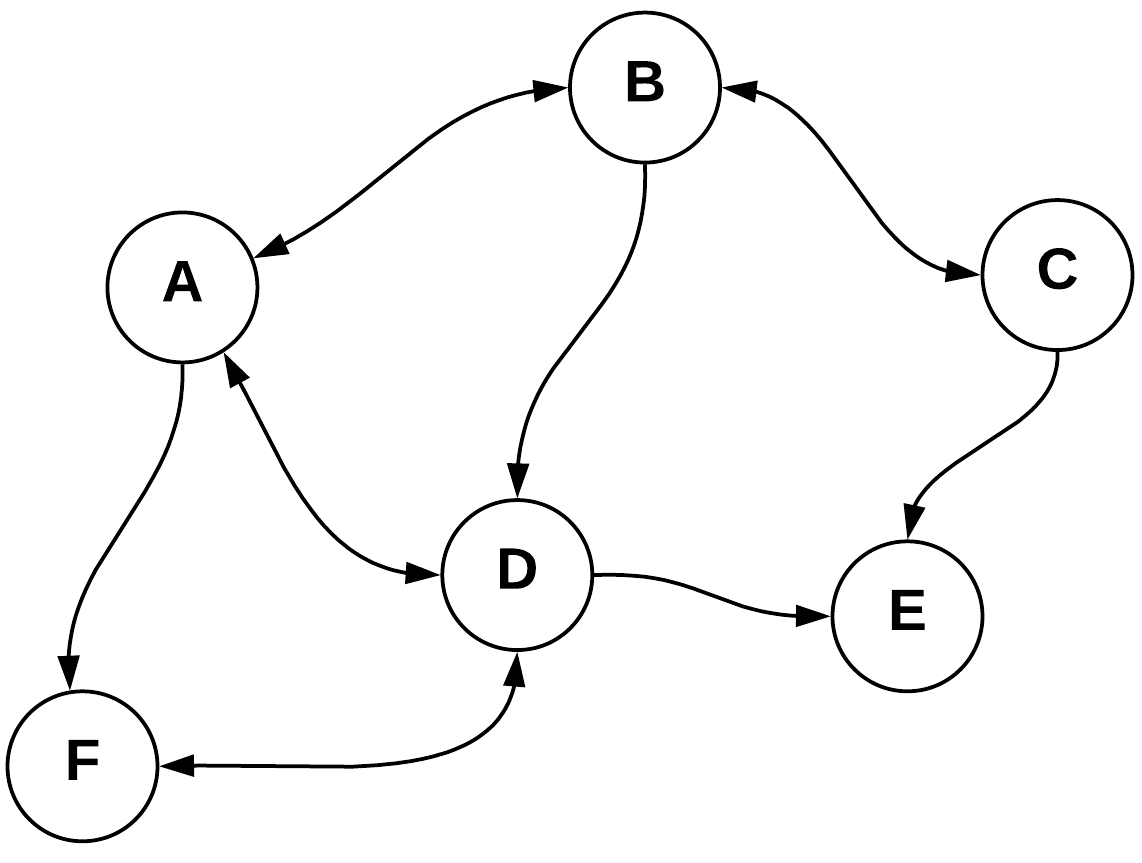
\includegraphics[width=0.5\columnwidth]{../figs/graph.png}
\end{center}
The above graph can be thought as a representation of different places in a city (represented by the nodes), and the lines with the arrows represent the roads connecting these different places. A line with two arrows allow two-way traffic, while line with single arrow only allow one way traffic. The connectivity between the different places can be summarized though the connectivity matrix $\mf{C} \in \mb{R}^{n \times n}$, where $n$ is the number of nodes in the graph. The elements of this connectivity matrix  represents whether or not there is a direct path between two places.
\[ 
c_{ij} = \begin{cases}
    1 & \text{there is a direct road between places } i \, \& \,j. \\
    0 & \text{otherwise.}
\end{cases}
\]
The diagonal element of $\mf{C}$ are zero, $c_{ii} = 0$.

Write down the connectivity matrix $\mf{C}$ for the graph shown above. How can we use the matrix $\mf{C}$ to answer the following questions? Explain exact matrix operation you would perform to answer these questions (Hint: Consider higher power of $\mf{C}$).
\begin{enumerate}
    \item Is there a path between two places $i$ and $j$ that goes via one other place? For example, we can go from $A$ to $D$ via $B$.
    \item How many paths are there between places $i$ and $j$ that goes via three other places?
\end{enumerate}

\end{enumerate}

\end{document}